\documentclass[12pt, oneside]{article}
\usepackage[utf8]{inputenc}
\usepackage{multirow}
\usepackage{physics}
\usepackage{float}
\usepackage{amsfonts}
\usepackage{graphicx}
\usepackage[english]{babel}
\usepackage{hyperref}
\usepackage{nicefrac}
\let\endtitlepage\relax
\usepackage{geometry}
    %\usepackage{showframe} %This line can be used to clearly show the new margins

\newgeometry{hmargin={24mm,24mm}}   % set the margins



\title{{\vspace{-1.5cm}}East-West Method Analysis over the All Triggers Dataset}
\author{E.Coronel,  S. Mollerach}
\date{February 2021}

\begin{document}

\begin{titlepage}
\maketitle
\end{titlepage}

En este capítulo se presentan los resultados obtenidos mediante el método East-West con los eventos de Todos los Disparos, para  distintos rangos de energía. Estos resultados se comparan con los valores obtenidos en \cite{Aab_2020} sobre los eventos  del Disparo Estándar. 
% \section{Tabla cantidad de eventos para distintos rangos de energía}

Los eventos son clasificados en los distintos rangos mediante la energía reportada por la Colaboración. El conjunto de eventos registrados con Todos los Disparos abarca los años 2014 y 2019, y para el Disparo Estándar se listan eventos medidos entre el 2004 y 2018. Las características de estos dos conjuntos de datos se especifican en la Tabla \ref{tab:datasets}

\begin{table}[H]
    \begin{small}
        \begin{center}
            \begin{tabular}{lc|l|l|l|}
\hline
\multicolumn{1}{|l|}{\multirow{4}{*}{\begin{tabular}[c]{@{}c@{}}Rango \\ Tiempo\end{tabular}}}    & Todos       & Inicio &\multicolumn{2}{l|}{1 de Enero, 2014 } \\ \cline{3-5} 
\multicolumn{1}{|l|}{}                                                                            & 6 años      & Fin    &\multicolumn{2}{l|}{1 de Enero, 2020} \\ \cline{2-5} 
\multicolumn{1}{|l|}{}                                                                            & Estándar    & Inicio &\multicolumn{2}{l|}{1 de Enero, 2004} \\ \cline{3-5}
\multicolumn{1}{|l|}{}                                                                            & 14.7 años   & Fin    &\multicolumn{2}{l|}{1 de Agosto, 2018} \\ \hline  \\

\hline                                                                          \multicolumn{2}{|c|}{Rango [EeV]}                                                    & \multicolumn{1}{c|}{0.25 - 0.5}  & \multicolumn{1}{c|}{ 0.5  - 1 } &\multicolumn{1}{c|}{ 1 - 2 } \\ \hline
\multicolumn{1}{|l|}{\multirow{2}{*}{Eventos}}                            & Todos    & $3\,967\,368$     & $3\,638\,226$   & $1\,081\,846$ \\ \cline{2-5} 
\multicolumn{1}{|l|}{}                                                    & Estándar & $770\,316$        & $2\,388\,467$   & $1\,243\,103$ \\ \hline
\multicolumn{1}{|l|}{\multirow{2}{*}{\begin{tabular}[c]{@{}c@{}}Energía \\ Media\end{tabular}}} & Todos    & $0.38$           & $0.69$         & $1.32$       \\ \cline{2-5} 
\multicolumn{1}{|l|}{}                                                                             & Estándar & $0.43$            & $0.70$          & $1.28$       \\ \hline
\end{tabular}
            \caption{Características de los conjuntos de datos para distintos rangos de energía }
            \label{tab:datasets}
        \end{center}
    \end{small}
\end{table}



\section{Resultados en distintos rangos de energía}
\subsection{Resultados en el rango 0.25 EeV - 0.5 EeV}

En la Tabla \ref{tab:primer_bin_data} se presentan los resultados para este rango de energía en las frecuencias solar y sidérea de Todos Los Disparos. Los mismos  se comparan con resultados con el Disparo Estándar que fueron reportados en \cite{Aab_2020}. Los valores de $\sigma$ de Todos los Disparos es la mitad que el valor reportado para el Disparo Estándar,  esto se debe a que el primer conjunto de datos tiene registrados $\sim 5$  veces más eventos que el segundo.

\begin{table}[H]
    \begin{small}
        \begin{center}
            \begin{tabular}[c]{l|c|c||c|}
\cline{2-4}                                       & \multicolumn{2}{c||}{Todos los disparos}    & \multicolumn{1}{c|}{Disparo Estándar}   \\ \hline
\multicolumn{1}{|l|}{Frecuencia:                } & Solar	                & Sidérea	                & Sidérea \cite{Aab_2020}   \\ \hline
\multicolumn{1}{|l|}{Amplitud r [\%]:           } & $0.17^{+0.22}_{-0.07}$	& $0.12^{+0.24}_{-0.03}$ 	& $0.5^{+0.4}_{-0.2}$ \cite{codigo}      \\
\multicolumn{1}{|l|}{$r_{99}$ [\%]:             } & \multicolumn{2}{c||}{0.58}                          & 1.1\cite{codigo}                 \\
\multicolumn{1}{|l|}{$r^{UL}$ [\%]:             } & 0.67 	                & 0.64                      & 1.4\cite{codigo}                 \\ 
\multicolumn{1}{|l|}{$\sigma$[\%]:              } & \multicolumn{2}{c||}{0.19}                          & 0.38\cite{codigo}       \\\hline
\multicolumn{1}{|l|}{Amplitud $d_\perp$[\%]:    } & -	                    & $0.16^{+0.31}_{-0.04}$ 	& $0.6^{+0.5}_{-0.3}$       \\
\multicolumn{1}{|l|}{$d_{99}$ [\%]:             } & - 	                    & 0.73                      & 1.5  \cite{codigo}                \\
\multicolumn{1}{|l|}{$d_{\perp}^{UL}[\%]$       } & -                       & 0.80                      & 1.8                         \\
\multicolumn{1}{|l|}{$\sigma_{x,y}$[\%]:        } & -	                    & 0.24	                    & 0.48       \\\hline
\multicolumn{1}{|l|}{Probabilidad      :        } & 0.66                    & 0.81	                    & 0.45       \\
\multicolumn{1}{|l|}{Fase[$^o$]:                } & 221$\pm$77              & 280$\pm$90                & 225$\pm$64\\ \hline
\multicolumn{1}{|l|}{$\langle\cos\delta \rangle$} & \multicolumn{2}{c||}{0.79}        	                & 0.79 \cite{codigo}        \\        
\multicolumn{1}{|l|}{$\langle\sin\theta \rangle$} & \multicolumn{2}{c||}{0.46}        	                & 0.52 \cite{codigo}        \\ \hline       
            \end{tabular}
            
        \end{center}
    \end{small}
    \caption{Características para las frecuencias solar y sidérea con el método East-West en el primer armónico en rango de energía 0.25 EeV - 0.5 EeV.}
    \label{tab:primer_bin_data}
\end{table}

\begin{figure}[H]
    \begin{small}
        \begin{center}
            \vspace*{-1. cm}
            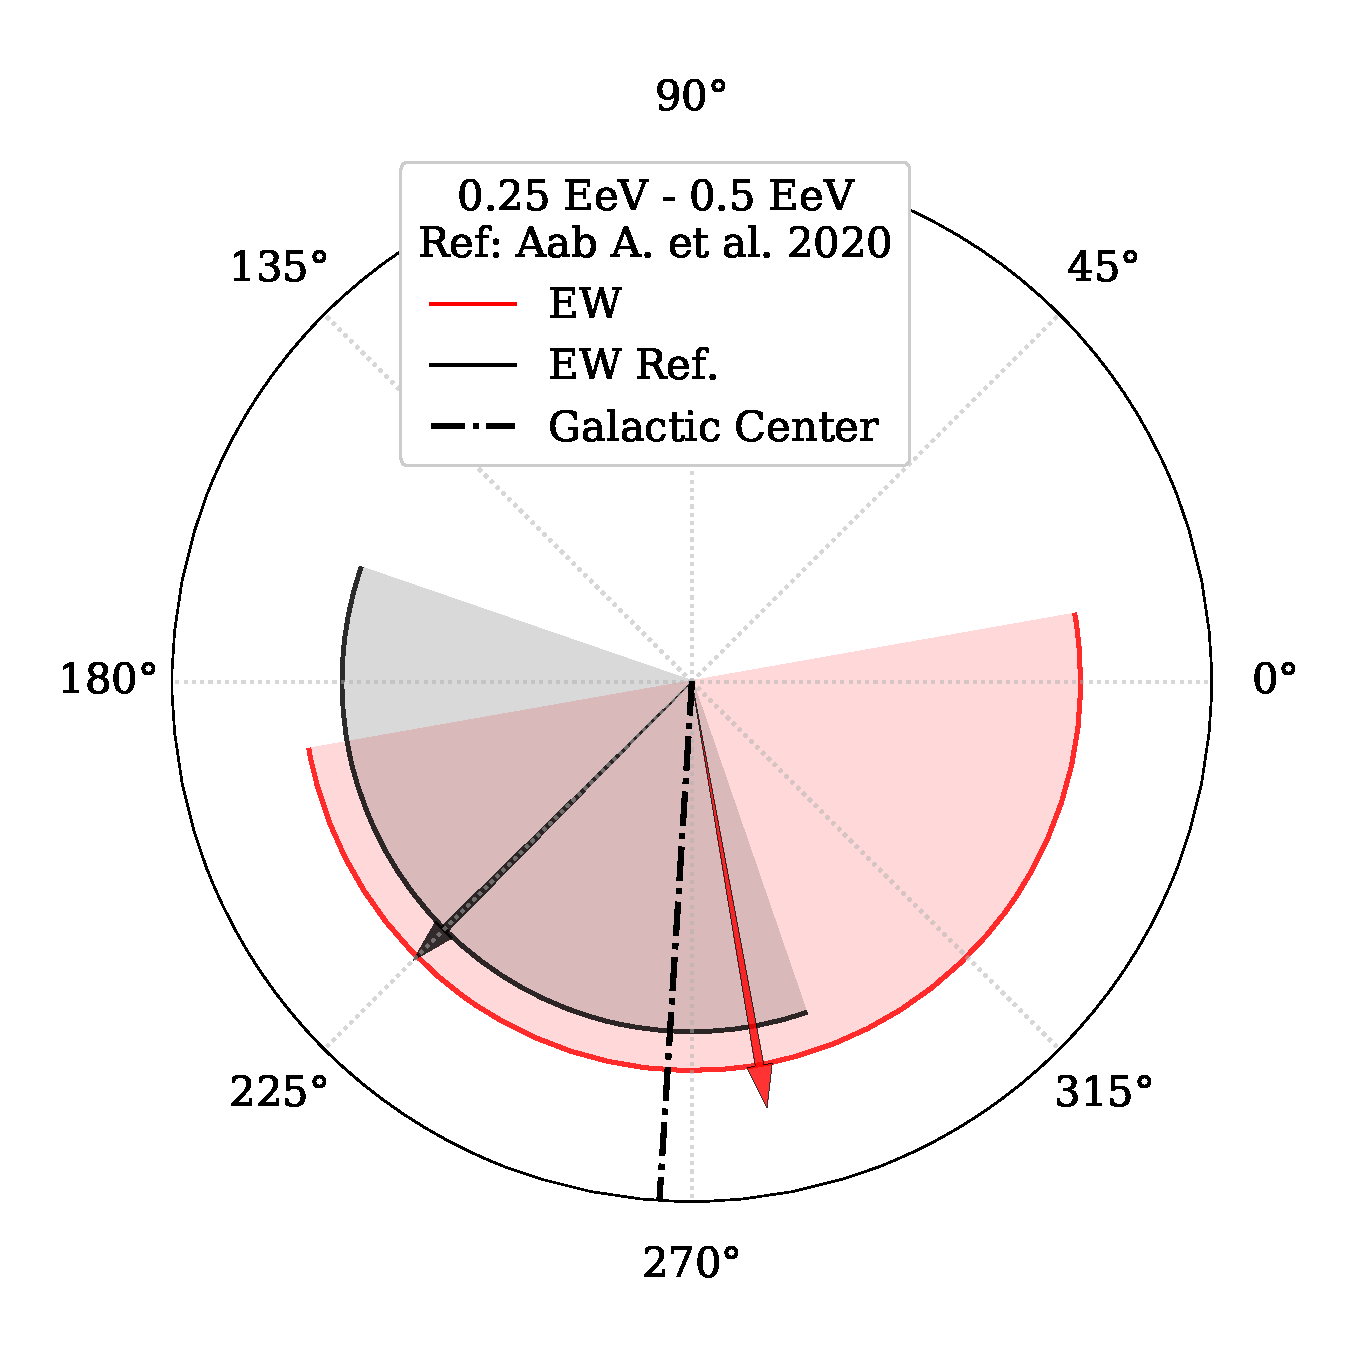
\includegraphics[width=0.65\textwidth]{Figs/phase_primer_bin_v3.pdf}
            \vspace*{-1 cm}
        \end{center}
        \caption{Valores de las fases obtenidos en este trabajo y en el trabajo Aab A. et al. (2020) \cite{Aab_2020} con sus respectivas incertidumbres para la frecuencia sidérea en el  rango 0.25 EeV - 0.5 EeV.}
        \label{fig:primer}
    \end{small}
\end{figure}

En la Fig. \ref{fig:primer} se comparan las  fases en frecuencia sidérea obtenida en este trabajo y la reportada en \cite{Aab_2020}, donde la línea punteada marca la dirección del centro galáctico.  En esta figura en la tabla anterior, se observa que la incertidumbre obtenida para la fase de Todos los Disparos es amplia, esto se debe a que la amplitud $r$ es pequeña comparada con el valor de $\sigma$. 


Realizando el barrido de frecuencias con la variable de la Ec.\ref{ra_arb}, se obtiene que en este rango de energía las amplitudes se  distribuyen en frecuencia como se muestra en la Fig.\ref{fig:primer_barrido}. La línea horizontal indica el valor de $r_{99}$ para cada frecuencia, además se observa que ninguna amplitud supera dicho umbral.



\begin{figure}[H]
    \begin{small}
        \begin{center}
            \vspace*{-0.6 cm}
            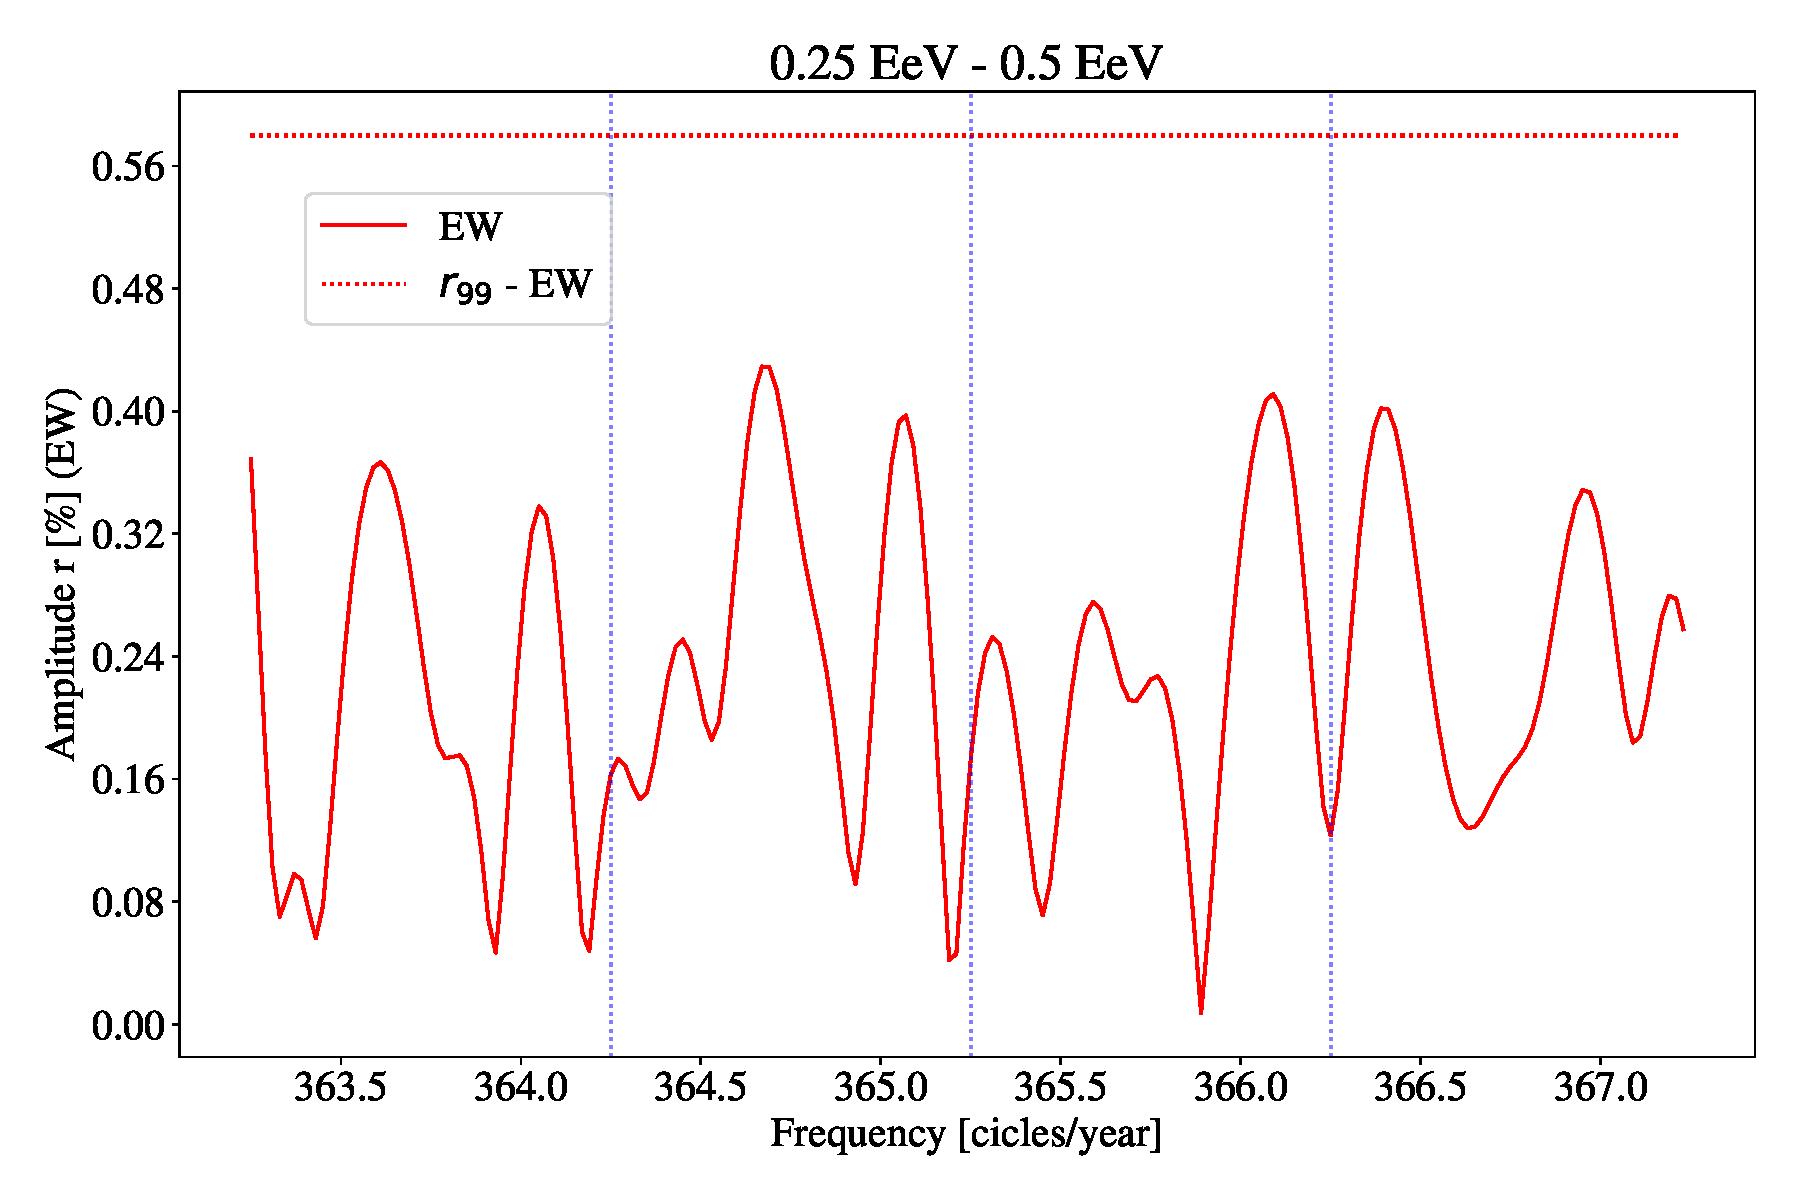
\includegraphics[width=0.9\textwidth]{Figs/plot_bin_1_barrido_v3_EW.pdf}
            \vspace*{-0.8 cm}
        \end{center}
        \caption{Barrido de frecuencias en el  rango 0.25 EeV - 0.50 EeV mediante el método East-West.}
        \label{fig:primer_barrido}
    \end{small}
\end{figure}

\subsection{Resultados en el rango 0.5 EeV - 1 EeV}
En la Tabla \ref{tab:primer_bin_data} se presentan los resultados para el rango 0.5 EeV - 1 EeV en las frecuencias solar y sidérea de Todos Los Disparos, además se comparan con los resultados reportados en \cite{Aab_2020}.


El barrido de frecuencias con la variable de la Ec.\ref{ra_arb} para este rango de energía se observa en la Fig.\ref{fig:segundo_barrido}. La línea horizontal indica el valor de $r_{99}$ para cada frecuencia, además se observa que ninguna frecuencia supera dicho umbral. 


En la Fig. \ref{fig:segundo} se comparan las direcciones en las que apuntan la fase en frecuencia sidérea obtenida en este trabajo con la obtenida en \cite{Aab_2020}. En esta figura se observa que resultados similares entre sí en valor e incertidumbre, y apuntan a una dirección cercana al centro galáctico.



\begin{table}[H]
        \begin{small}
            \begin{center}
                \begin{tabular}[c]{l|c|c||c|}
\cline{2-4}                                       & \multicolumn{2}{c||}{Todos los disparos}    & \multicolumn{1}{c|}{Disparo Estándar}   \\ \hline
\multicolumn{1}{|l|}{Frecuencia:                } & Solar	                & Sidérea	                & Sidérea \cite{Aab_2020}   \\ \hline
\multicolumn{1}{|l|}{Amplitud r [\%]:           } & $0.43^{+0.21}_{-0.14}$	& $0.44^{+0.21}_{-0.14}$ 	& $0.38^{+0.20}_{-0.14}$ \cite{codigo}      \\
\multicolumn{1}{|l|}{$r_{99}$ [\%]:             } & \multicolumn{2}{c||}{0.56}                          & 0.64\cite{codigo}                 \\
\multicolumn{1}{|l|}{$r^{UL}$ [\%]:             } & 0.89 	                & 0.90                      & 0.90 \cite{codigo}                 \\ 
\multicolumn{1}{|l|}{$\sigma$[\%]:              } & \multicolumn{2}{c||}{0.18}                          & 0.21 \cite{codigo}      \\\hline
\multicolumn{1}{|l|}{Amplitud $d_\perp$[\%]:    } & -	                    & $0.56^{+0.27}_{-0.18}$ 	& $0.5^{+0.3}_{-0.2}$       \\
\multicolumn{1}{|l|}{$d_{99}$ [\%]:             } & - 	                    & 0.71                      & 0.8   \cite{codigo}                \\
\multicolumn{1}{|l|}{$d_{\perp}^{UL}[\%]$       } & -                       & 1.1                       & 1.1                         \\
\multicolumn{1}{|l|}{$\sigma_{x,y}$[\%]:        } & -	                    & 0.23	                    & 0.21       \\\hline
\multicolumn{1}{|l|}{Probabilidad      :        } & 0.065                   & 0.055	                    & 0.20       \\
\multicolumn{1}{|l|}{Fase[$^o$]:                } & 205$\pm$34              & 258$\pm$34                & 261$\pm$43\\ \hline
\multicolumn{1}{|l|}{$\langle\cos\delta \rangle$} & \multicolumn{2}{c||}{0.79}        	                & 0.79 \cite{codigo}        \\        
\multicolumn{1}{|l|}{$\langle\sin\theta \rangle$} & \multicolumn{2}{c||}{0.50}        	                & 0.54\cite{codigo}        \\ \hline       
                \end{tabular}
            \end{center}
        \end{small}
        \caption{Características para las frecuencias solar y sidérea con el método East-West en el primer armónico en rango de energía 0.5 EeV - 1 EeV}
        \label{tab:segundo_bin_data}
    \end{table}


    


    \begin{figure}[H]
        \begin{small}
            \begin{center}
                \vspace*{-1.6 cm}
                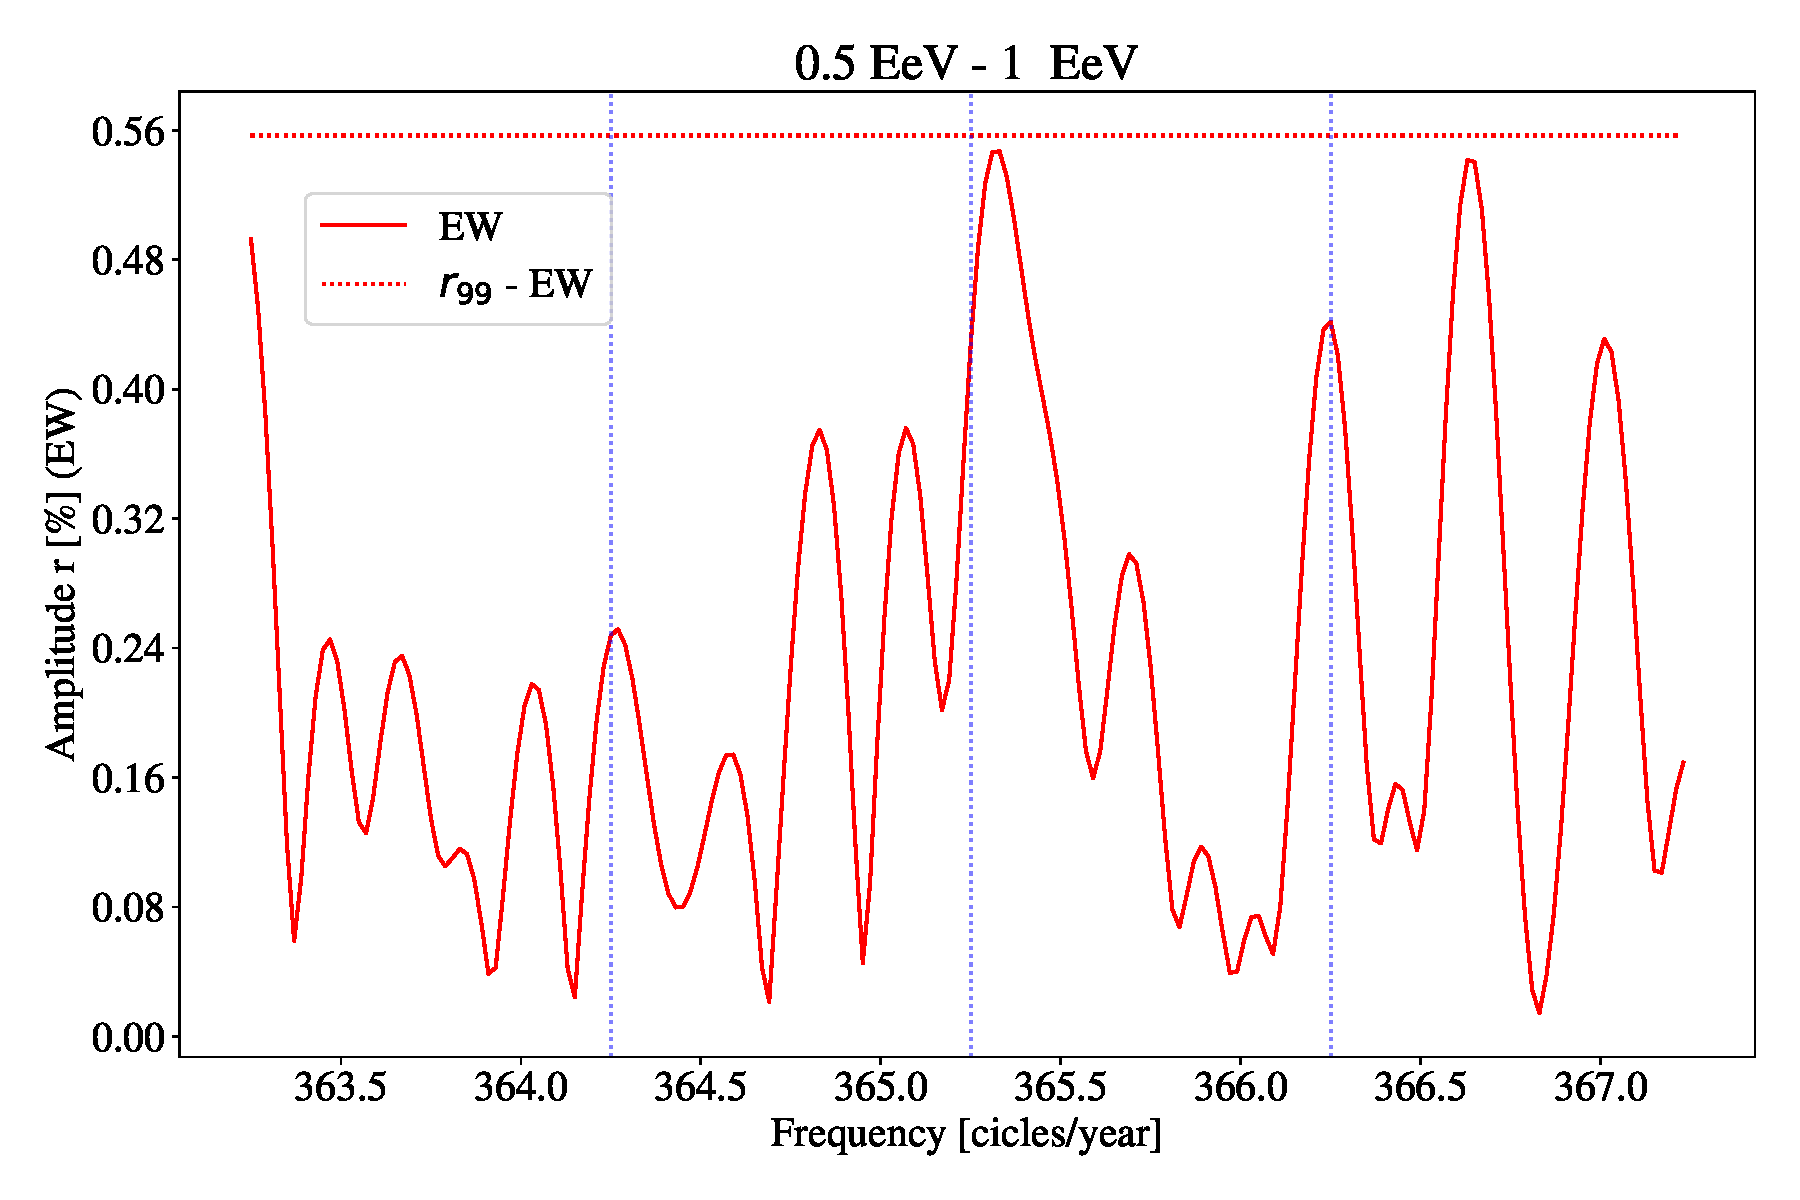
\includegraphics[width=0.9\textwidth]{Figs/plot_bin_2_barrido_v3_EW.pdf}
                \vspace*{-0.6 cm}
            \end{center}
            \caption{Barrido de frecuencias en el  rango 0.5 EeV - 1.0 EeV mediante el método East-West.}
            \label{fig:segundo_barrido}
        \end{small}
    \end{figure}    

\subsection{Resultados en el rango 1 EeV - 2 EeV}

 
En las Tablas \ref{tab:solar_3}  se comparan los resultados de este trabajo  para la frecuencia solar. Las amplitudes están por debajo de $r_{99}$ y son compatibles entre sí.


    \begin{figure}[H]
        \begin{small}
            \begin{center}
                \vspace*{-0.65 cm}
                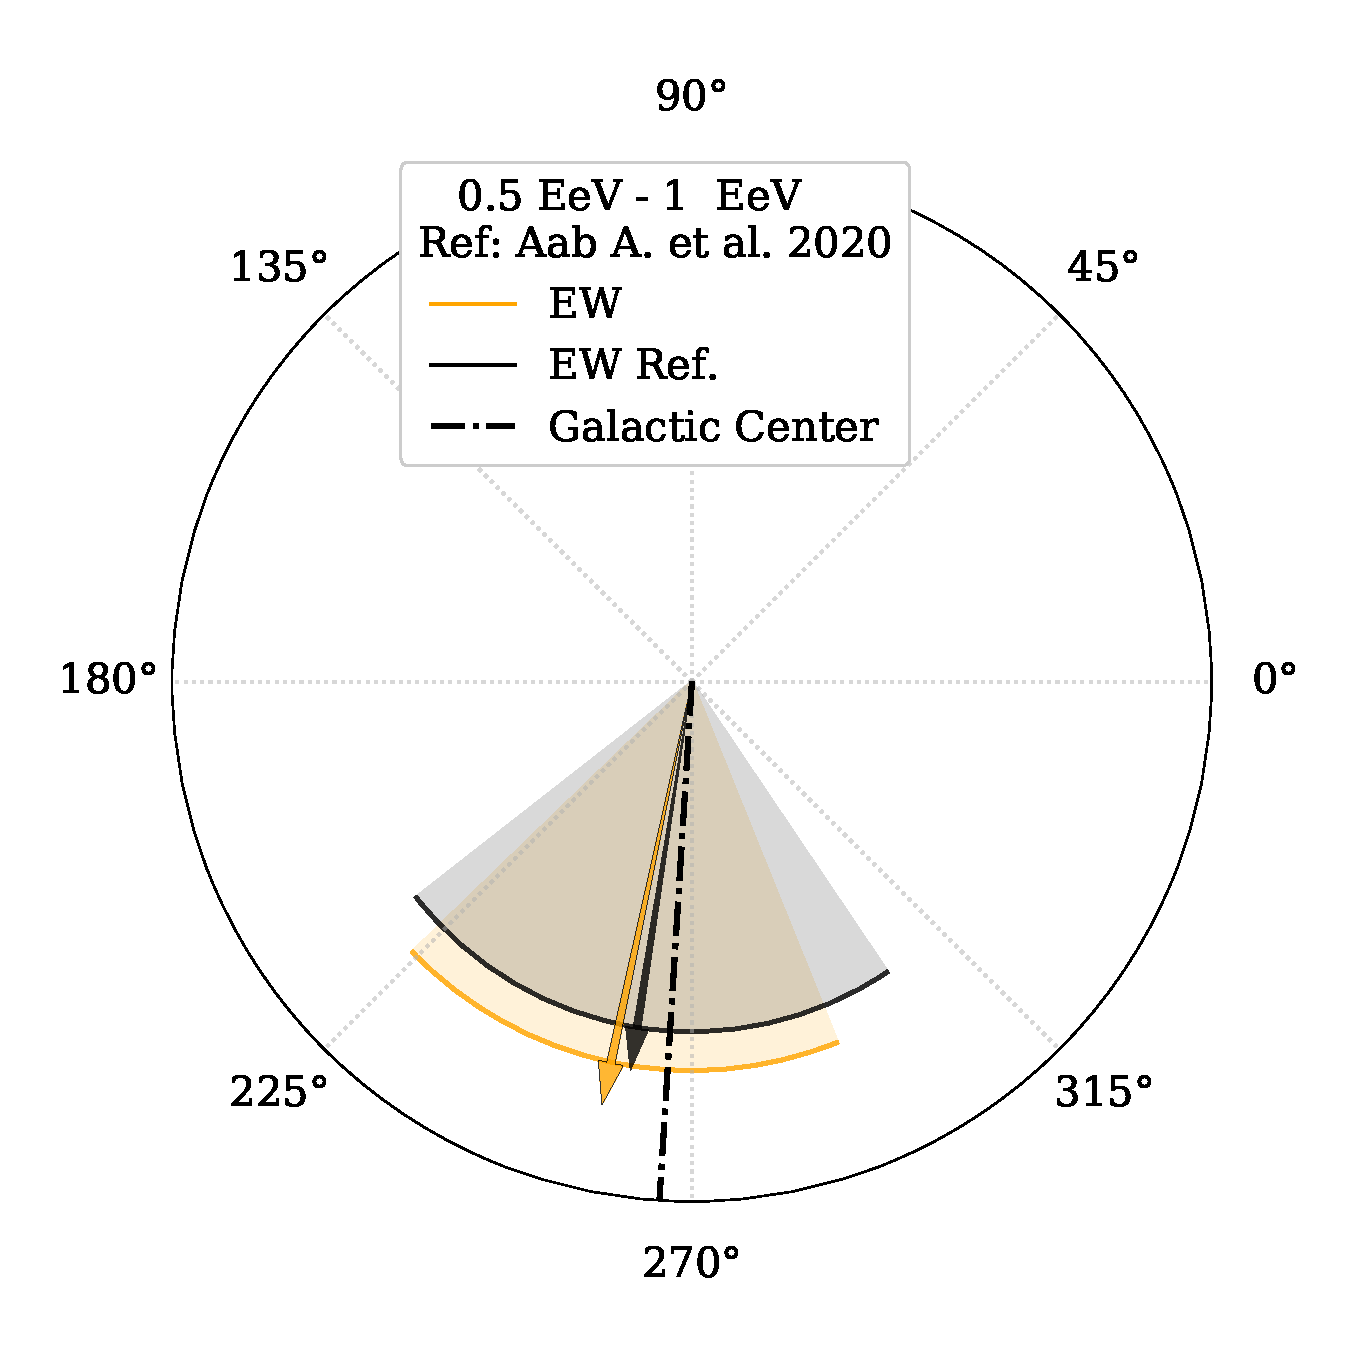
\includegraphics[width=0.65\textwidth]{Figs/phase_segundo_bin_v3.pdf}
                \vspace*{-1.1 cm}
            \end{center}
            \caption{Valores de las fases obtenidos en este trabajo y en el trabajo Aab A.  et al. (2020) \cite{Aab_2020} con sus respectivas incertidumbres para la frecuencia sidérea en el rango 0.5 EeV - 1.0 EeV .}
            \label{fig:segundo}
        \end{small}
    \end{figure}


    \begin{table}[H]
        \vspace*{-0.81 cm}
        \begin{small}
            \begin{center}
                \begin{tabular}[c]{l|c|c|c|}
                    \cline{2-4}         & \multicolumn{3}{c|}{Todos los disparos} \\ \cline{2-4}
                                        & Rayleigh   &                   & East - West            \\\hline
\multicolumn{1}{|l|}{Frecuencia:}       & \multicolumn{3}{c|}{Solar}        \\
\multicolumn{1}{|l|}{Amplitud $r$[\%]:} & $0.24^{+0.16}_{-0.09}$&         & $0.28^{+0.35}_{-0.11}$ \\
\multicolumn{1}{|l|}{$r_{99}$ [\%]:   } & 0.41                  &         & 0.91       \\
\multicolumn{1}{|l|}{$r_{UL}$ [\%]:   } & 0.58                  &        & 1.1       \\
\multicolumn{1}{|l|}{$\sigma$:        } & 0.14                  &         & 0.30          \\\hline
\multicolumn{1}{|l|}{Probabilidad:    } & 0.22                  &          & 0.65          \\
\multicolumn{1}{|l|}{Fase:            } & 260$\pm$48            &         & 279$\pm$76    \\\hline
                \end{tabular}
            \end{center}
            \vspace*{-0.41 cm}
        \end{small}
        \caption{Características para la frecuencia solar con los métodos de Rayleigh  e East-West en el primer armónico en el rango 1 EeV - 2 EeV.}
        \label{tab:solar_3}
    \end{table}
    


    En la Tabla \ref{tab:siderea_3} se comparan los resultados de este trabajo y los obtenidos en el trabajo \cite{Aab_2020} para la frecuencia sidérea. Para Todos los Disparos se comparan los métodos de Rayleigh y East-West, en el primer método se obtiene que la probabilidad que la amplitud obtenida se deba al ruido es de $6.3\%$ mientras que en segundo método $26\%$. Esta diferencia entre probabilidades no puede deberse a la cantidad de eventos, porque es el mismo conjunto de datos. En la Fig.\ref{fig:tercer} se observan en una figura en coordenadas polares mostrando las fases del trabajo \cite{Aab_2020} y este trabajo para la frecuencia sidérea.


    El barrido de frecuencias con la variable de la Ec.\ref{ra_arb} para este rango de energía se observa en la Fig.\ref{fig:tercer_barrido}. La línea horizontal indica el valor de $r_{99}$ para cada frecuencia y se observa que ninguna frecuencia supera dicho umbral. En la frecuencia solar no se observa ningún pico, esto se debe a que el método East - West es robusto con respecto a las modulación del clima. Se observa un pico en sidérea pero el mismo no es significativo con respecto al $r_{99}$.


    \begin{figure}[H]
        \begin{small}
            \begin{center}
                \vspace*{-0.65 cm}
                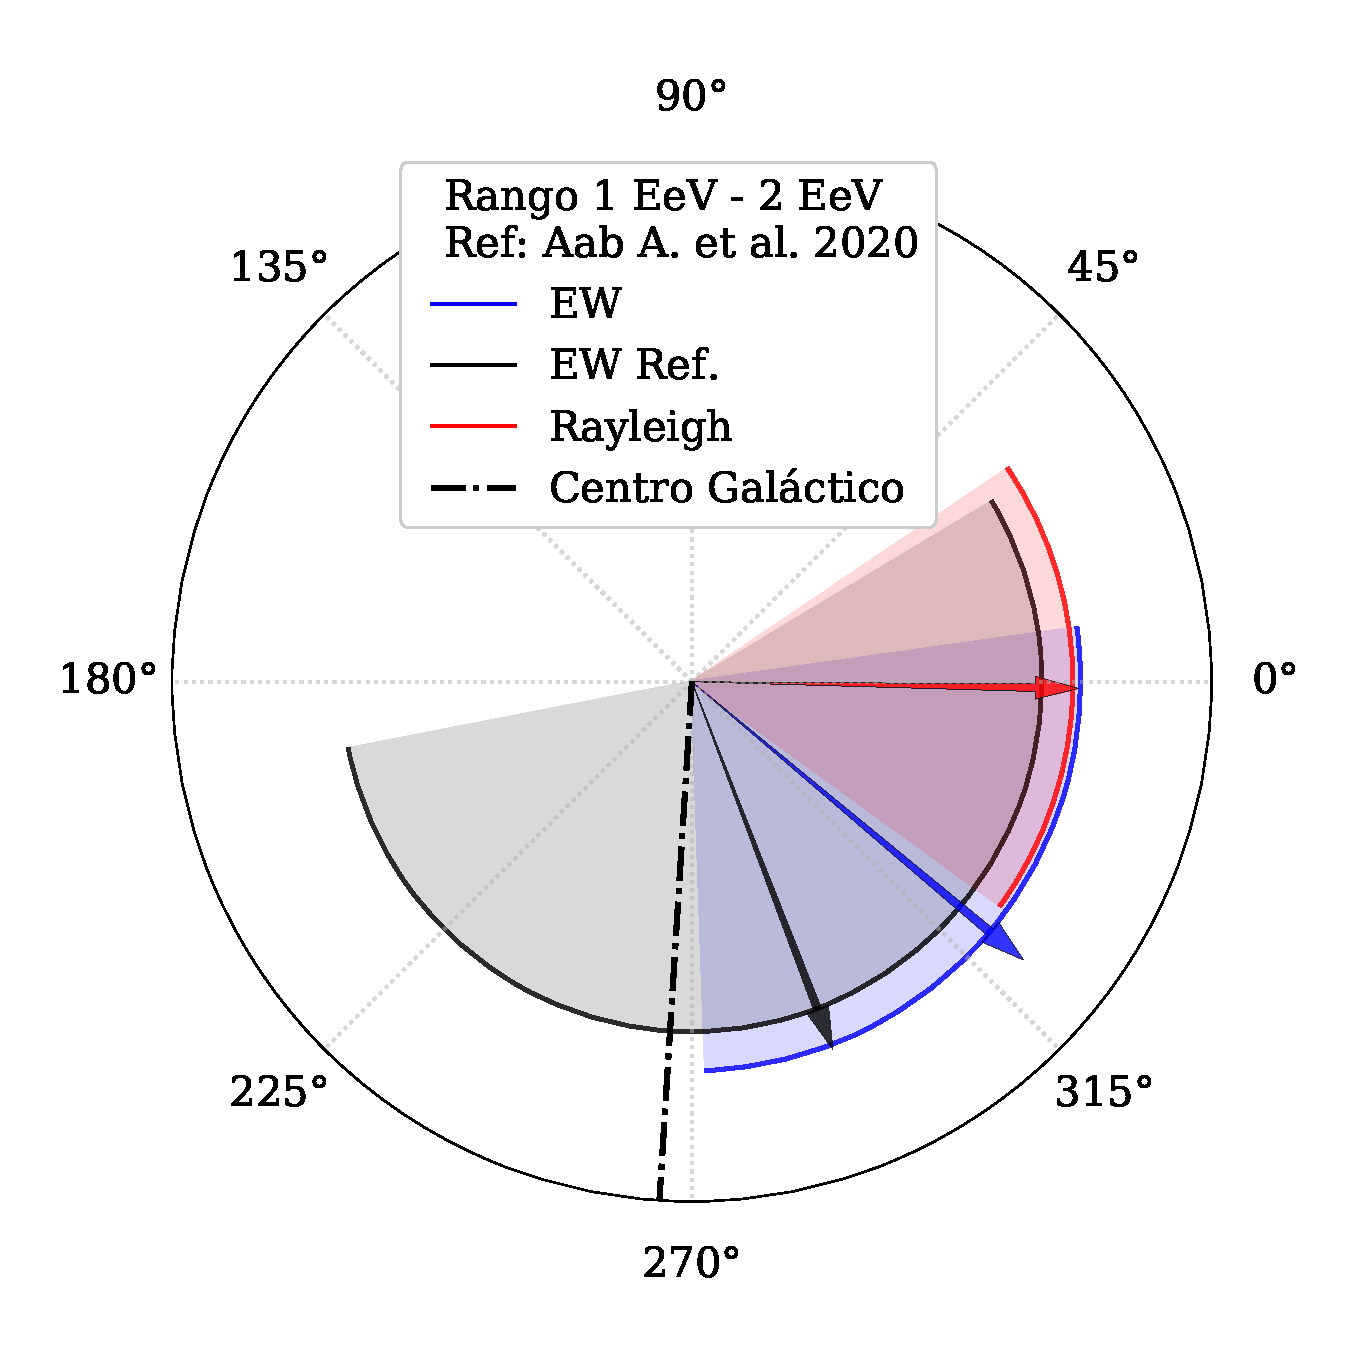
\includegraphics[width=0.65\textwidth]{Figs/phase_tercer_bin_v3.pdf}
                \vspace*{-1.2 cm}
            \end{center}
        \caption{Valores de las fases obtenidos en este trabajo y en el trabajo Aab A. et al. (2020) \cite{Aab_2020} con sus respectivas incertidumbres para la frecuencia sidérea en el  rango 1.0 EeV - 2.0 EeV .}
        \label{fig:tercer}
        \end{small}
    \end{figure}
    \begin{table}[H]
        \vspace*{-0.51 cm}
        \begin{small}
            \begin{center}
                \begin{tabular}[c]{l|c|c|c||c|}
                    \cline{2-5}                 & \multicolumn{3}{c||}{Todos los Disparos}                  & Disparo Estándar      \\
                    \cline{2-5}                 & Rayleigh               &       & East - West                 & East - West\cite{Aab_2020}      \\\hline
\multicolumn{1}{|l|}{Frecuencia:             }  & \multicolumn{3}{c||}{Sidérea}                               & Sidérea        \\ \hline
\multicolumn{1}{|l|}{Amplitud $r$ [\%]:      }  & $0.32^{+0.16}_{-0.10}$ &  	    & $0.5^{+0.3}_{-0.2}$         & $0.14^{+0.37}_{-0.02}$\cite{codigo}       \\
\multicolumn{1}{|l|}{$r_{99}$[\%]:           }  & 0.41	                 &         & 0.91                        & 0.84\cite{codigo}        \\
\multicolumn{1}{|l|}{$r^{UL}[\%]$      }        & 0.66                   &         & 1.3                         & 0.89 \cite{codigo}        \\
\multicolumn{1}{|l|}{$\sigma$[\%]:     }        & 0.14                   &         & 0.30	                    & 0.28 \cite{codigo}          \\ \hline
\multicolumn{1}{|l|}{Amplitud $d_\perp$ [\%]:}  & $0.41^{+0.20}_{-0.13}$ &         & $0.6^{+0.4}_{-0.3}$         & $0.18^{+0.47}_{-0.02}$       \\ 
\multicolumn{1}{|l|}{$d_{99}$[\%]:           }  & 0.53	                 &        & 1.1                         & 1.1\cite{codigo}        \\
\multicolumn{1}{|l|}{$d_{\perp}^{UL}[\%]$    }  & 0.84                   &         & 1.6                         & 1.1        \\
\multicolumn{1}{|l|}{$\sigma_{x,y}$[\%]:     }  & 0.17                   &         & 0.38	                    & 0.35          \\ \hline
\multicolumn{1}{|l|}{Probabilidad:           }  & 0.063	                 &            & 0.26                        & 0.87          \\
\multicolumn{1}{|l|}{Fase[$^o$]:             }  & 357$\pm$35             &        & 320$\pm$48                 & 291$\pm$100      \\\hline
\multicolumn{1}{|l|}{$\langle\cos\delta\rangle$}&{0.78}&  &{0.78}                        & 0.78       \\        
\multicolumn{1}{|l|}{$\langle\sin\theta\rangle$}&{0.55}&  &{0.55}                        & 0.57       \\ \hline       
\end{tabular}
            \end{center}
        \end{small}
        \vspace*{-0.21 cm}
        \caption{Características para la frecuencia sidérea con los métodos de Rayleigh  e East-West en el primer armónico en el rango 1 EeV - 2 EeV.}
        \label{tab:siderea_3}
    \end{table}



    \begin{figure}[H]
        \begin{small}
            \begin{center}
                \vspace*{-0.21 cm}
                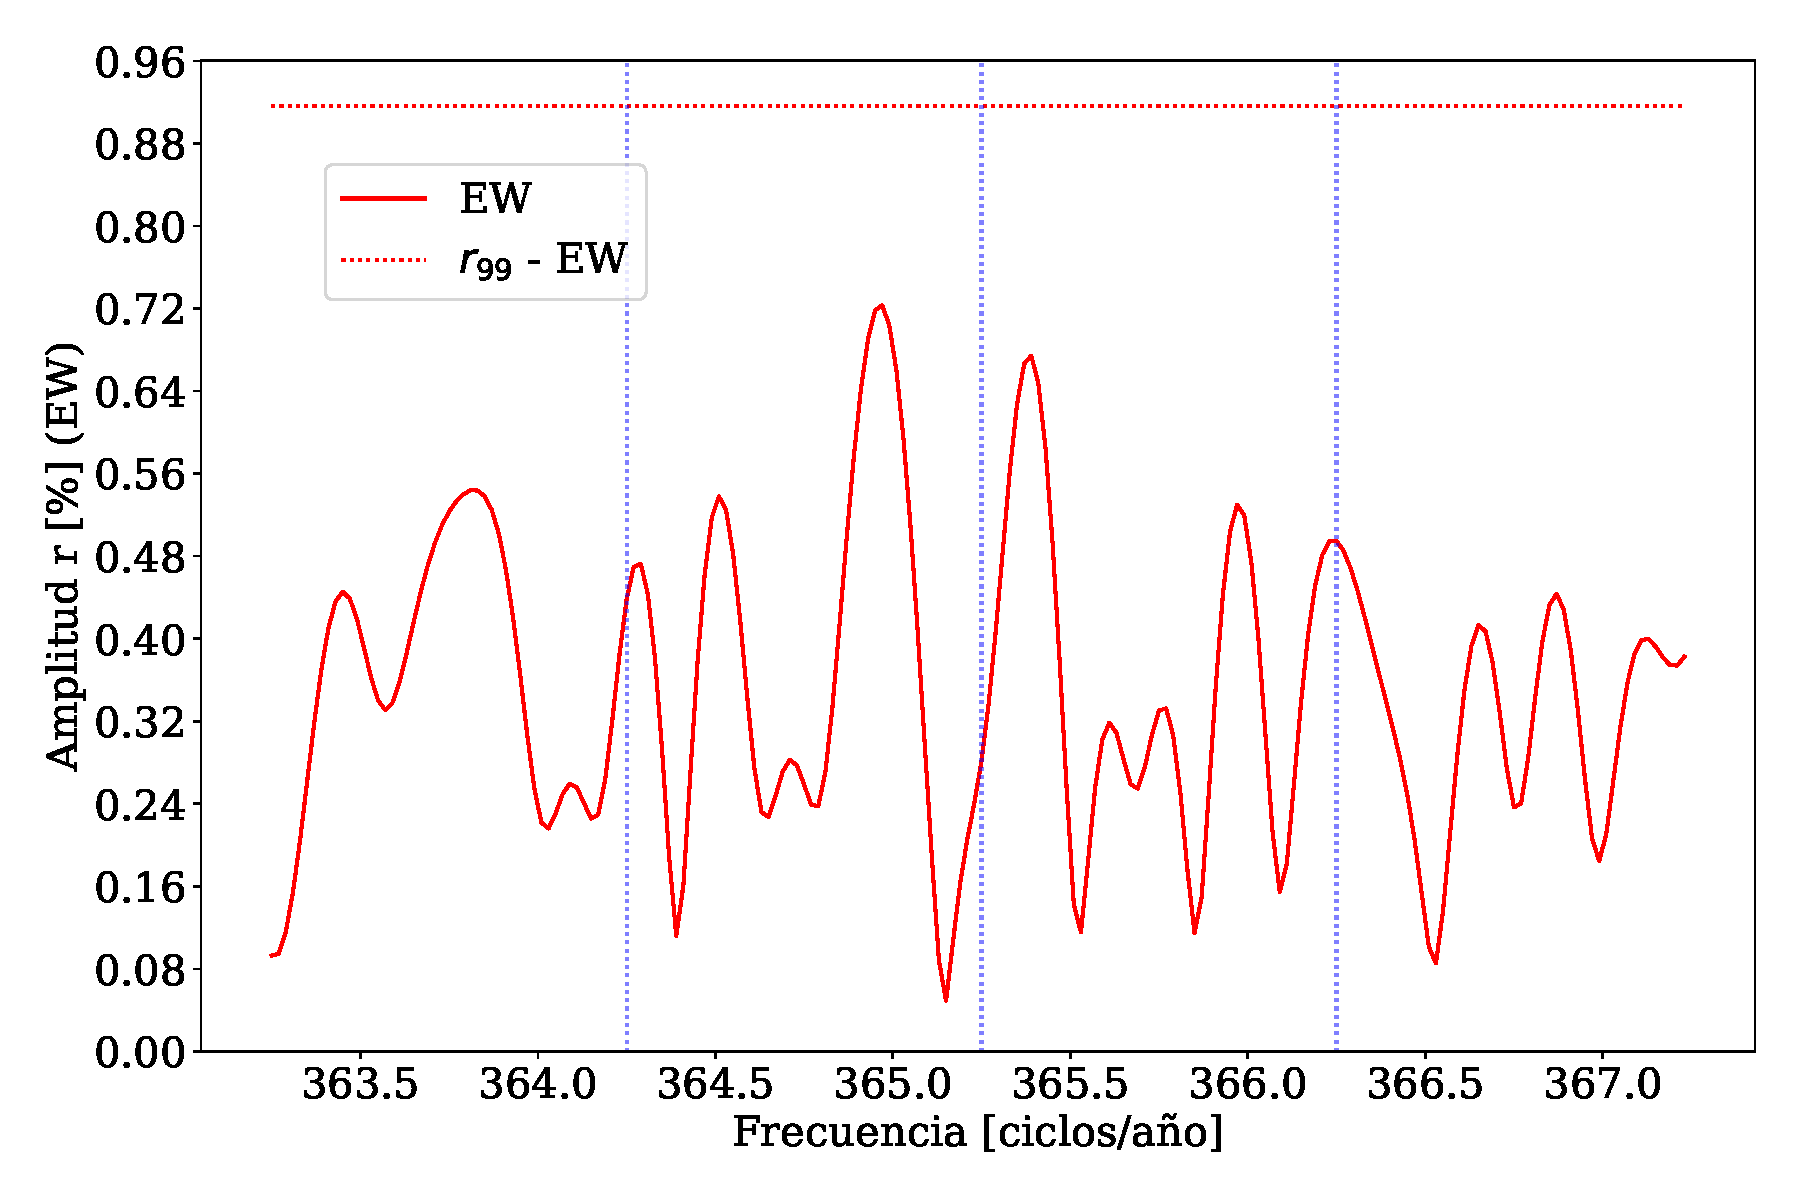
\includegraphics[width=0.9\textwidth]{Figs/plot_bin_3_barrido_v3_EW.pdf}
                \vspace*{-1 cm}
            \end{center}
            \caption{Barrido de frecuencias en el rango 1 EeV - 2 EeV mediante el método East-West.}
            \label{fig:tercer_barrido}
        \end{small}
    \end{figure}    


    \section{Análisis de los resultados}

    El barrido de frecuencias para el conjunto de datos de Todos los Disparos contiene datos de 6 años. Este rango de tiempo  permite tener una resolución de $\sim\nicefrac{1}{6}  \,$ciclos/año \cite{resolucion_barrido}. Los picos obtenidos en los barridos presentados en las Figs.\ref{fig:primer_barrido}, \ref{fig:segundo_barrido} y \ref{fig:tercer_barrido} están distanciados en promedio $\nicefrac{1}{5}\,$ciclos/año entre sí por lo que están dentro de la resolución posible del análisis. 

    % Para poder comparar los resultados de $d_\perp$ entre sí, podríamos graficar los valores de la proyección y de la límite del $99\%$ como se muestra en la Fig.\ref{fig:no_normalizado}. El inconveniente es la cantidad de datos en cada rango de energía entre los conjuntos de datos, Todos los Disparos y Disparo Estándar, son distintos.

    % \begin{figure}[H]
    %     \begin{small}
    %         \begin{center}
    %             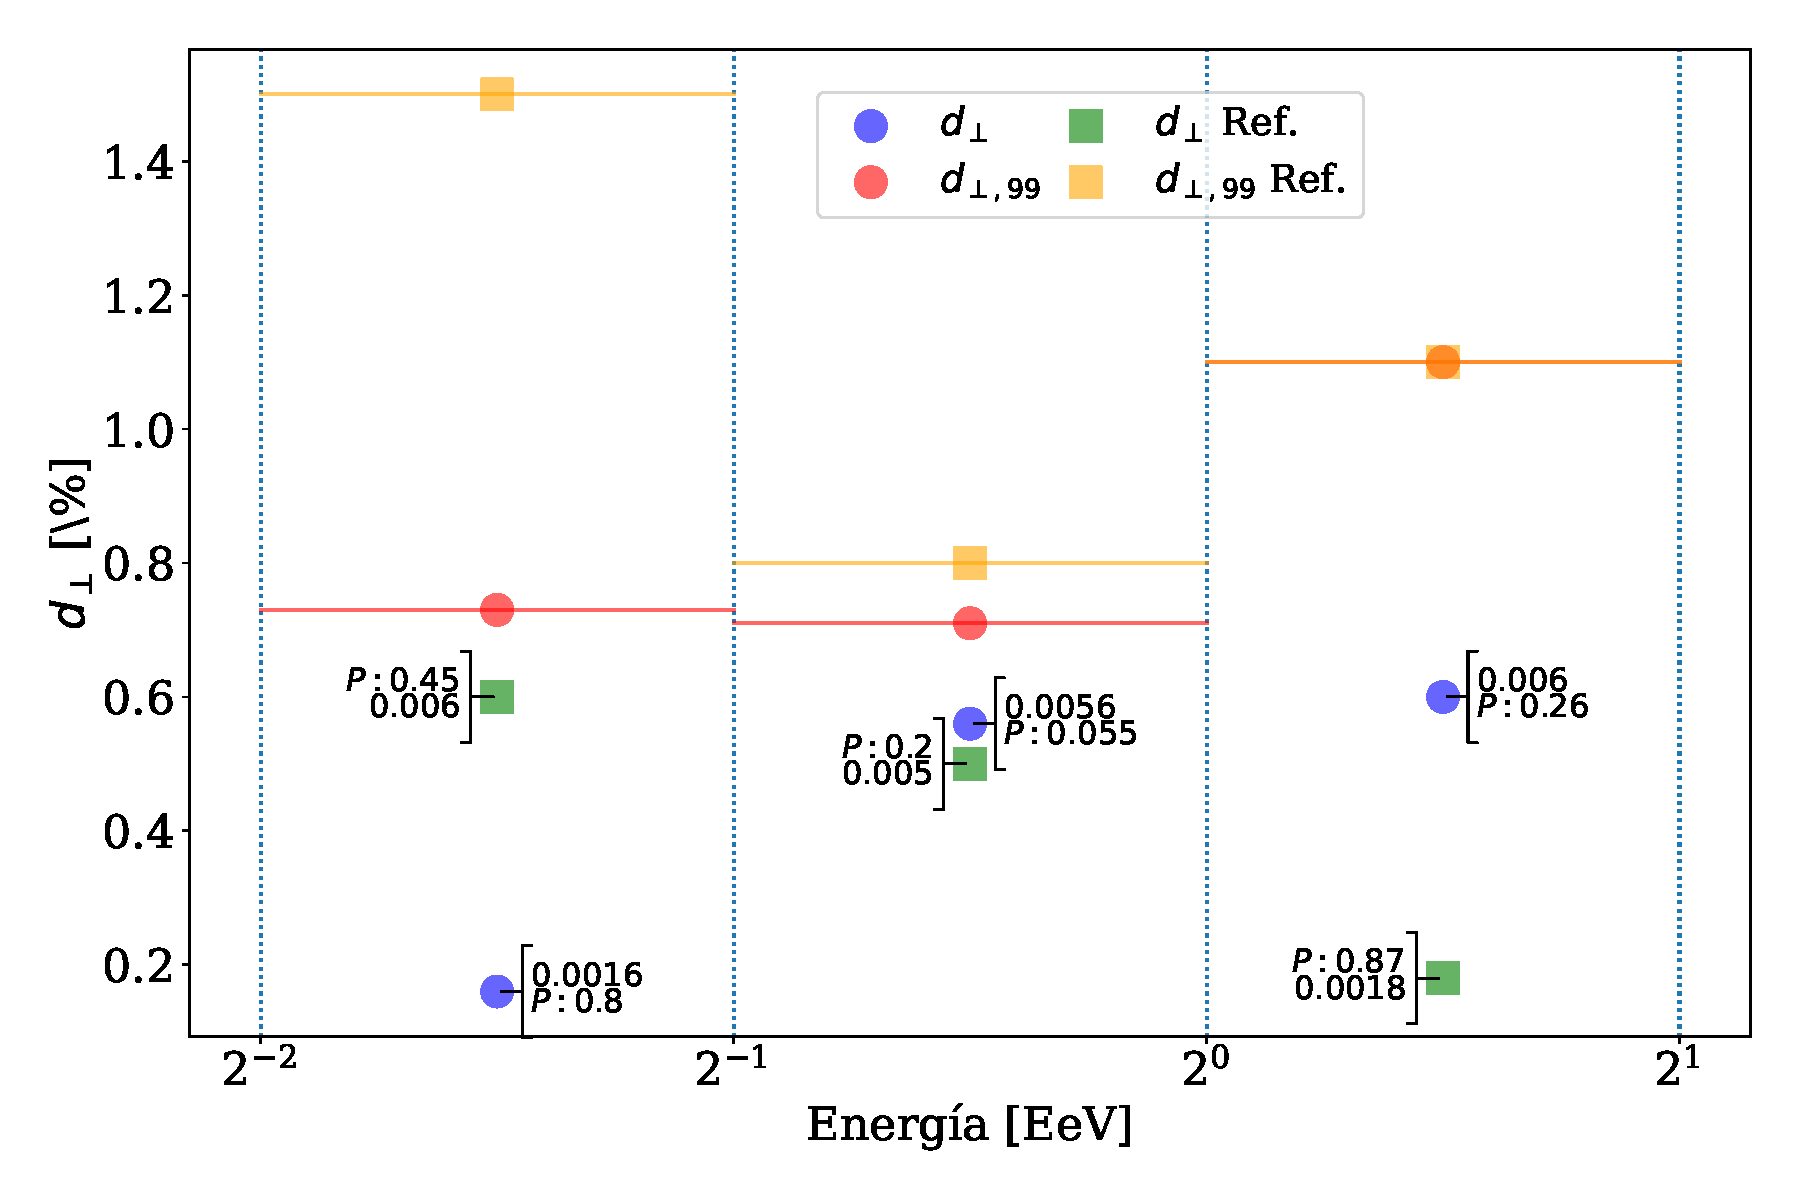
\includegraphics[width=0.75\textwidth]{Figs/d_perp_no_normalizado_v4.pdf}
    %         \end{center}
    %         \caption{Sin normalizar}
    %         \label{fig:no_normalizado}
    %     \end{small}
    % \end{figure}
    
    % Para compararlos mejor con respecto a $d_{\perp,UL}$, usamos el valor de cada rango y de cada conjunto de datos, para normalizar la amplitud de $d_{\perp,UL}$. Como se muestra en la Fig.\ref{fig:normalizado}, ahora $d_{\perp,UL}=1$ y los otros valores se pueden comparar. 

    % \begin{figure}[H]
    %     \begin{small}
    %         \begin{center}
    %             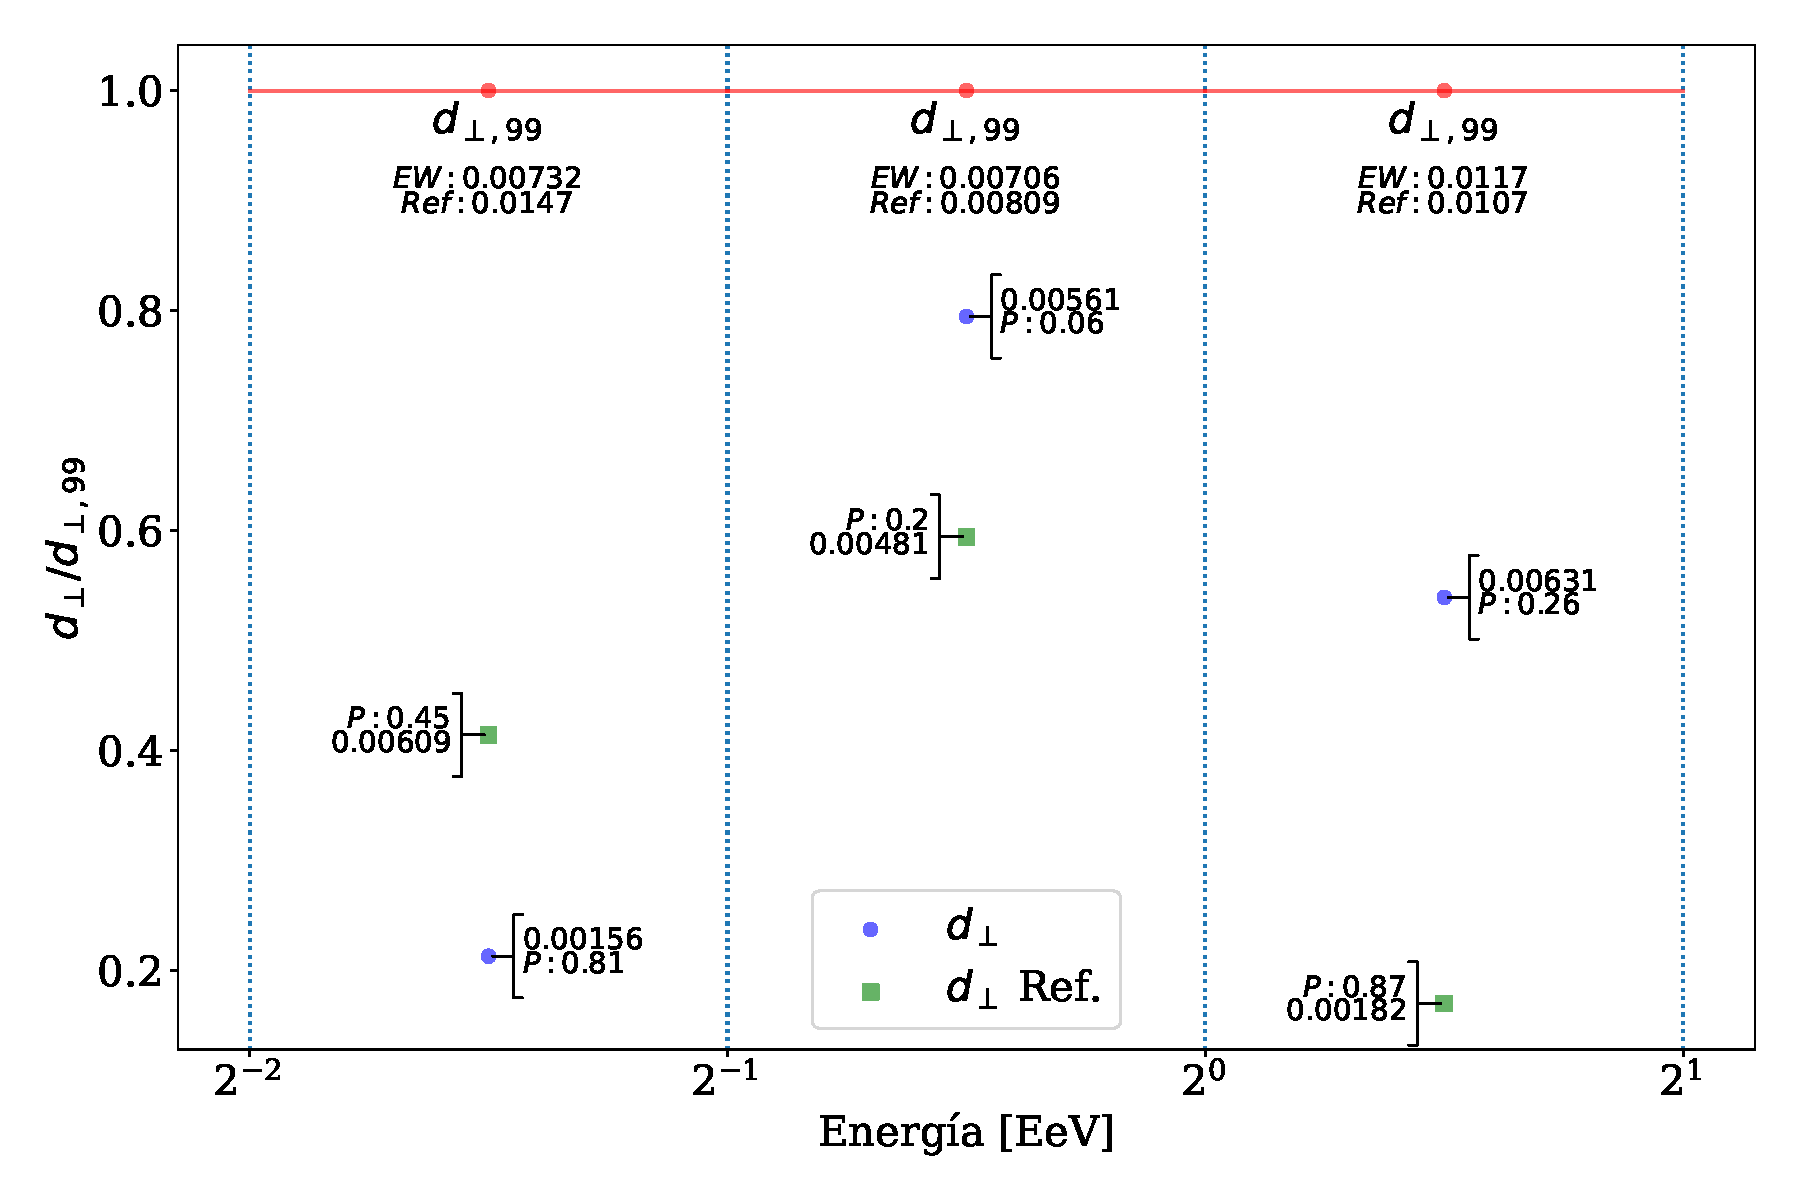
\includegraphics[width=0.75\textwidth]{Figs/d_perp_normalizado.pdf}
    %         \end{center}
    %         \caption{Valores normalizados con $d_{\perp,UL}$}
    %         \label{fig:normalizado}
    %     \end{small}
    % \end{figure}

    Una forma  para poder comparar los resultados de $d_\perp$ calculados de distintos conjuntos de  datos entre sí, es dividir estos valores con  sus respectivos $\sigma_{x,y}$. De esta manera, podemos comparar cuan apartados están con respecto $\sigma_{x,y}$. De esta manera se obtiene la Fig.\ref{fig:normalizado_sigma}, donde podemos decir que en los rangos entre 0.5 EeV - 1.0 EeV y 1.0 EeV - 2.0 EeV, la amplitud obtenida en este trabajo utilizando los eventos de Todos los Disparos es más significativa que los resultados obtenidos por el trabajo \cite{Aab_2020} con el Disparo Estándar. Estos resultados difieren de trabajo \cite{Aab_2020} por $\sim 1\sigma_{x,y}$ y $\sim 2 \sigma_{x,y}$ respectivamente. Para comparar los resultados en el  rango 0.25 EeV - 0.5 EeV, tenemos que tener en cuenta que el Disparo Estándar tiene una sensibilidad menor que el Todos los Disparos. Esto se ve claramente en la Tabla \ref{tab:datasets}, donde el primero tiene 7 veces menos eventos para analizar que el segundo. Por lo tanto, la discrepancia entre este trabajo y los resultados presentados en \cite{Aab_2020} puede deberse a la  diferencia de eventos a estudiar causada por la sensibilidad del disparo.

    \begin{figure}[H]
        \begin{small}
            \begin{center}
                \vspace*{-0.21 cm}
                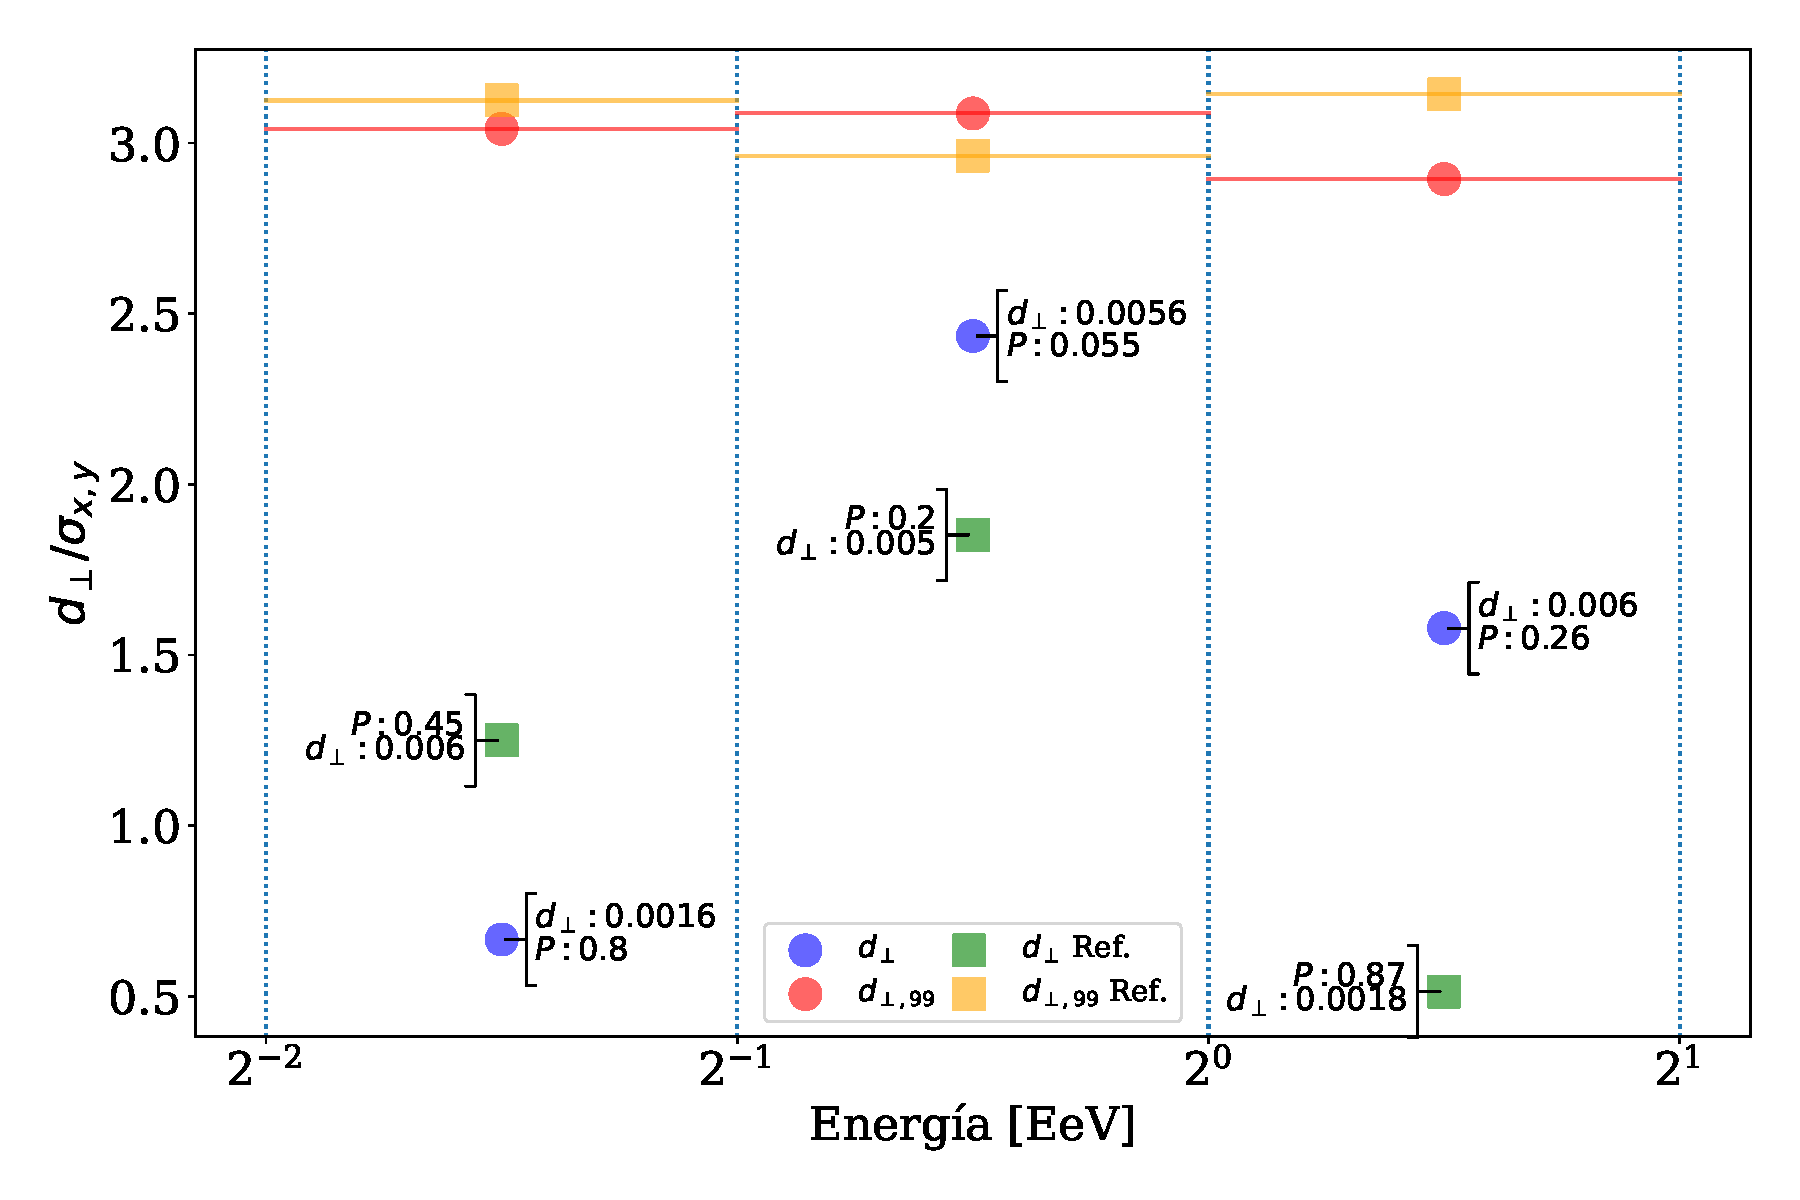
\includegraphics[width=\textwidth]{Figs/d_perp_normalizado_sigmas_v6.pdf}
                \vspace*{-1 cm}
            \end{center}
            \caption{Variaciones de la amplitud $d_\perp$ con respecto a $\sigma_{x,y}$ comparados con $d_{\perp,99}$ para distintos rangos de energía. Estos valores son obtenidos con el método East-West. }
            \label{fig:normalizado_sigma}
        \end{small}
    \end{figure}



    Considerando los valores de $\sigma_{x,y}$ y $d_\perp$ obtenidos para cada rango de energía y con los métodos Rayleigh y East-West, es posible  comparar las direcciones, valores e incertidumbres en la Fig.\ref{fig:incertidumbre}. Las líneas punteadas están centradas en los valores reportados  en cada rango de energía por el trabajo \cite{Aab_2020}, obtenido con el Disparo Estándar. El  radio de cada círculo punteado igual al $\sigma_{x,y}$ de cada rango de energía. Los círculos sombreados indican el rango de incertidumbre  a $1\sigma_{x,y}$ de los valores obtenidos en este trabajo utilizando Todos los Disparos. Cada flecha dentro de estos círculos sombreados indica a dirección y valor de $d_\perp$.    El punto asociado al método Rayleigh corregido con la modulación del clima de Todos los Disparos en el rango 1-2 EeV se denota con \emph{Ray,mod}.


    En los rangos de energía 0.25 EeV - 0.5 EeV y 0.5 EeV - 1.0 EeV, los valores obtenidos con Todos los Disparos y el Disparo Estándar son compatibles entre sí dentro de la incertidumbre, además de contener la dirección al centro galáctico dentro de sus incertidumbres. Esto es interesante de resaltar ya que es esos rangos de energía, se espera que los rayos cósmicos sean galácticos.

    En el rango 1.0 EeV - 2.0 EeV, se comparan resultados para el método de Rayleigh (\emph{Ray}) y el método East-West (\emph{EW}) obtenidos con Todos los Disparos, y el valor obtenido por la Colaboración en el trabajo \cite{Aab_2020} mediante el método Rayleigh con el Disparo Estándar. Todos estos resultados son compatibles entre sí dentro de $1\sigma_{x,y}$ de incertidumbre. 

\begin{figure}[H]
    \begin{small}
        \begin{center}
            \vspace*{-0.21 cm}
            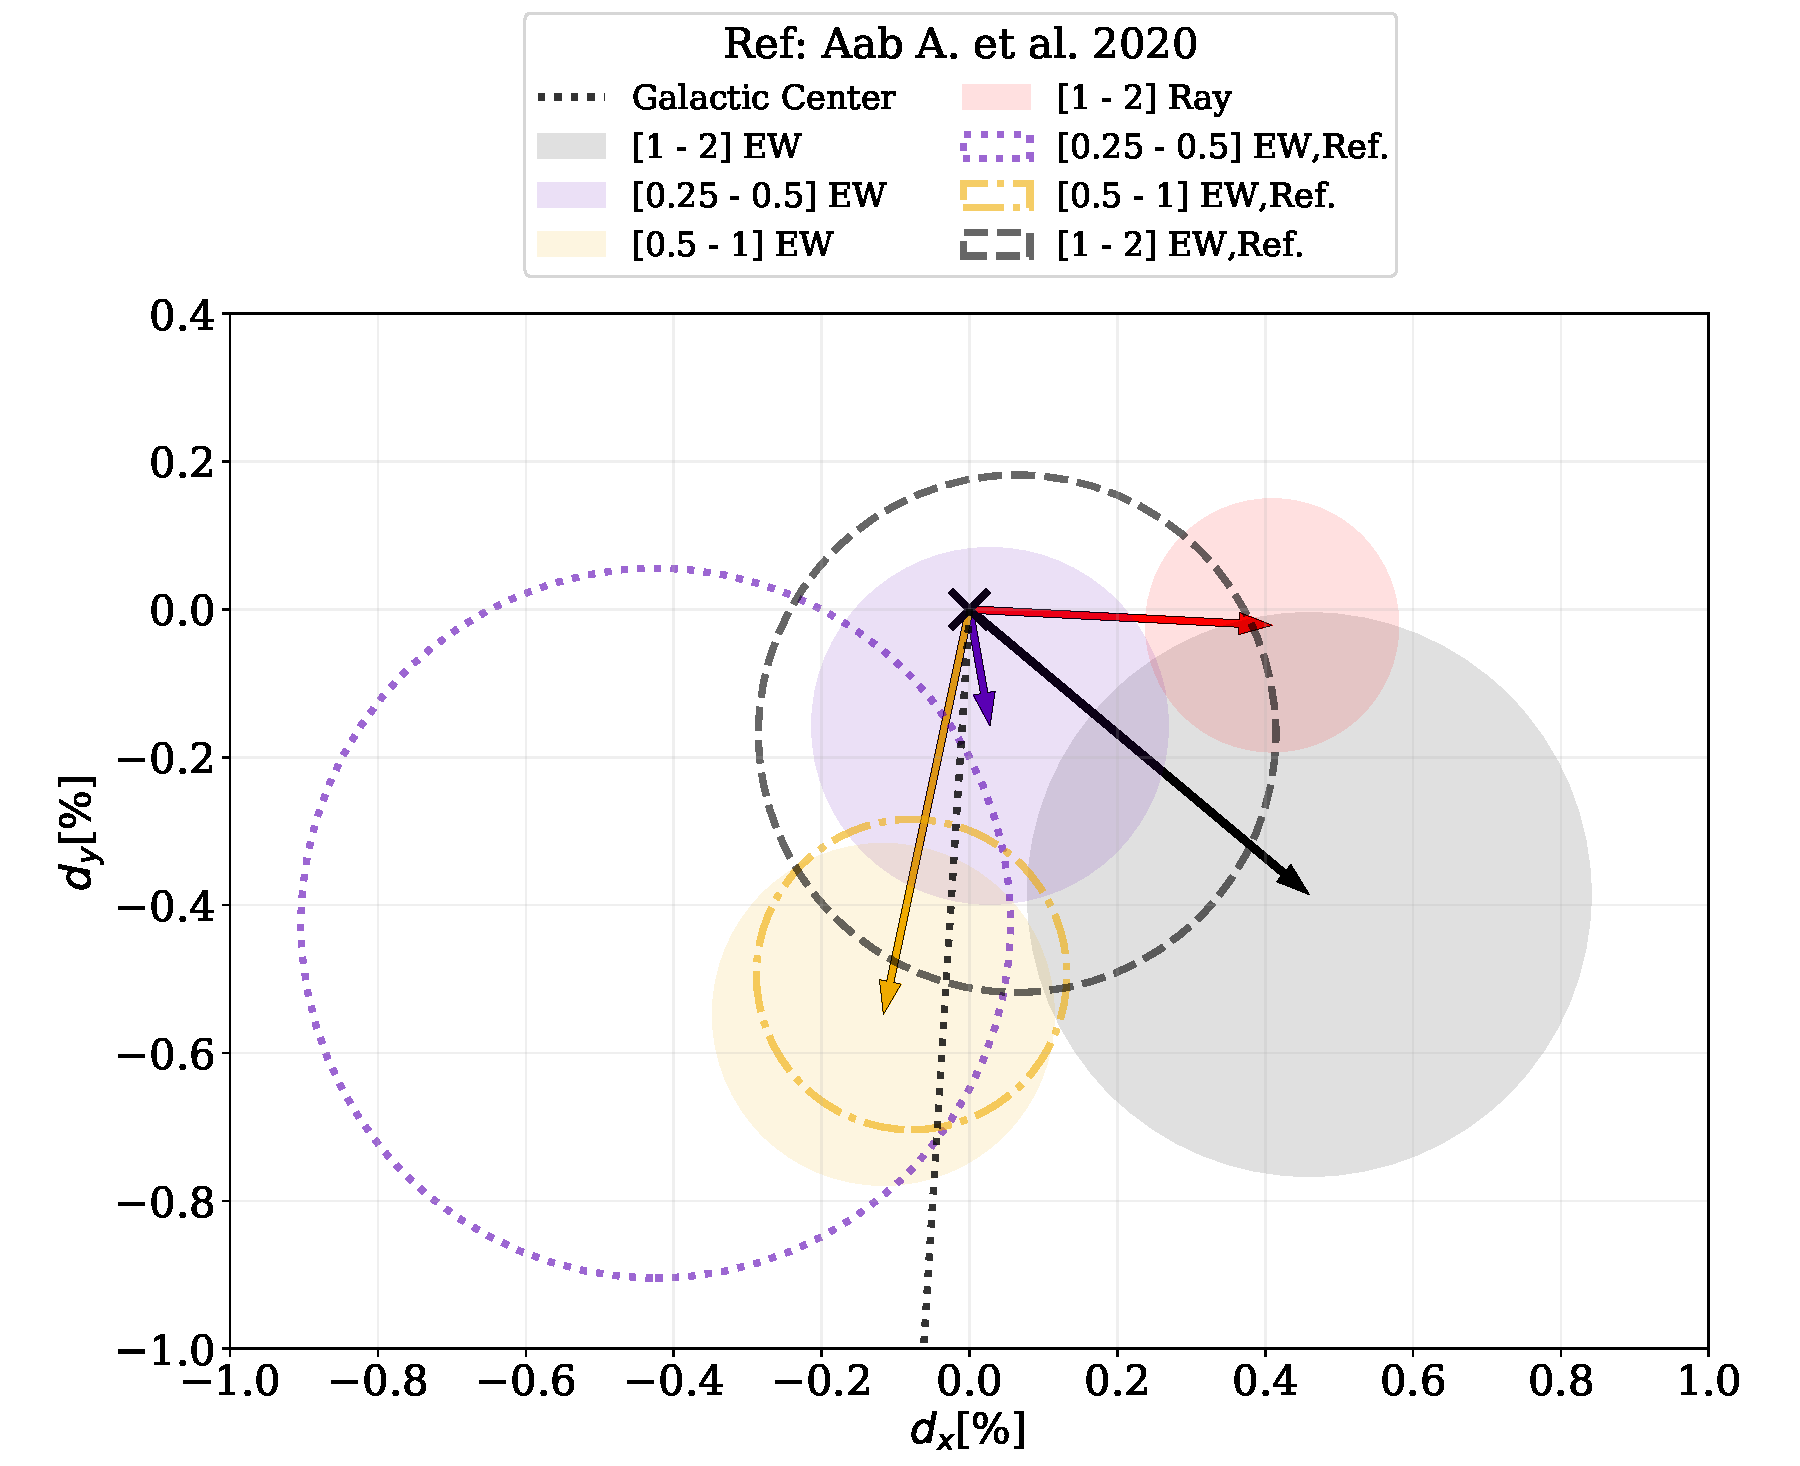
\includegraphics[width=\textwidth]{Figs/comparando_sigmas_v4.pdf}
            \vspace*{-1. cm}
        \end{center}
        \caption{Amplitudes con incertidumbre, apuntando en la dirección  de la fase. Los círculos punteados los valores del trabajo Aab A. et al. (2020) \cite{Aab_2020} con sus respectivas incertidumbres y la línea punteada en negro marca la dirección del centro galáctico.}
        \label{fig:incertidumbre}
    \end{small}
\end{figure}



\begin{thebibliography}{9}
    \bibitem{Aab_2020}
    {Aab A. et al.},{Cosmic-Ray Anisotropies in Right Ascension Measured by the {Pierre   Auger Observatory}}.
    \emph{The Astrophysical Journal}, \textbf{891}~(2), 142, 2020. \url{https://doi.org/10.3847/1538-4357/ab7236}.
    \bibitem{codigo}  
    {Code used in \cite{Aab_2020}}.
\end{thebibliography}
    

\end{document}